\documentclass[tikz,border=8pt]{standalone}
% Shared look for every TikZ diagram. Load with % Shared look for every TikZ diagram. Load with % Shared look for every TikZ diagram. Load with \input{../../tools/tikz-style.tex}
\usepackage[T1]{fontenc}
\usepackage{lmodern}
\renewcommand{\sfdefault}{lmr}  % diagrams use the same serif as the text
\usetikzlibrary{arrows.meta, positioning, shapes.geometric, calc, fit, backgrounds}
\definecolor{cblue}{HTML}{4C78A8}
\definecolor{corange}{HTML}{F58518}
\definecolor{cgreen}{HTML}{54A24B}
\definecolor{cred}{HTML}{E45756}
\definecolor{cpurple}{HTML}{B279A2}
\definecolor{cgrey}{HTML}{6B6B6B}
\tikzset{
  every picture/.style={font=\sffamily, line width=1.2pt},
  box/.style={draw=#1, fill=#1!12, rounded corners=4pt, align=center, inner sep=7pt, minimum height=1.1cm},
  box/.default=cgrey,
  arrow/.style={-{Stealth[length=3mm]}, draw=cgrey, line width=1.4pt},
  title/.style={font=\sffamily\bfseries\Large},
  note/.style={font=\sffamily\small, text=cgrey, align=center},
}
\AtBeginDocument{\hyphenpenalty=10000 \exhyphenpenalty=10000}

\usepackage[T1]{fontenc}
\usepackage{lmodern}
\renewcommand{\sfdefault}{lmr}  % diagrams use the same serif as the text
\usetikzlibrary{arrows.meta, positioning, shapes.geometric, calc, fit, backgrounds}
\definecolor{cblue}{HTML}{4C78A8}
\definecolor{corange}{HTML}{F58518}
\definecolor{cgreen}{HTML}{54A24B}
\definecolor{cred}{HTML}{E45756}
\definecolor{cpurple}{HTML}{B279A2}
\definecolor{cgrey}{HTML}{6B6B6B}
\tikzset{
  every picture/.style={font=\sffamily, line width=1.2pt},
  box/.style={draw=#1, fill=#1!12, rounded corners=4pt, align=center, inner sep=7pt, minimum height=1.1cm},
  box/.default=cgrey,
  arrow/.style={-{Stealth[length=3mm]}, draw=cgrey, line width=1.4pt},
  title/.style={font=\sffamily\bfseries\Large},
  note/.style={font=\sffamily\small, text=cgrey, align=center},
}
\AtBeginDocument{\hyphenpenalty=10000 \exhyphenpenalty=10000}

\usepackage[T1]{fontenc}
\usepackage{lmodern}
\renewcommand{\sfdefault}{lmr}  % diagrams use the same serif as the text
\usetikzlibrary{arrows.meta, positioning, shapes.geometric, calc, fit, backgrounds}
\definecolor{cblue}{HTML}{4C78A8}
\definecolor{corange}{HTML}{F58518}
\definecolor{cgreen}{HTML}{54A24B}
\definecolor{cred}{HTML}{E45756}
\definecolor{cpurple}{HTML}{B279A2}
\definecolor{cgrey}{HTML}{6B6B6B}
\tikzset{
  every picture/.style={font=\sffamily, line width=1.2pt},
  box/.style={draw=#1, fill=#1!12, rounded corners=4pt, align=center, inner sep=7pt, minimum height=1.1cm},
  box/.default=cgrey,
  arrow/.style={-{Stealth[length=3mm]}, draw=cgrey, line width=1.4pt},
  title/.style={font=\sffamily\bfseries\Large},
  note/.style={font=\sffamily\small, text=cgrey, align=center},
}
\AtBeginDocument{\hyphenpenalty=10000 \exhyphenpenalty=10000}

\begin{document}
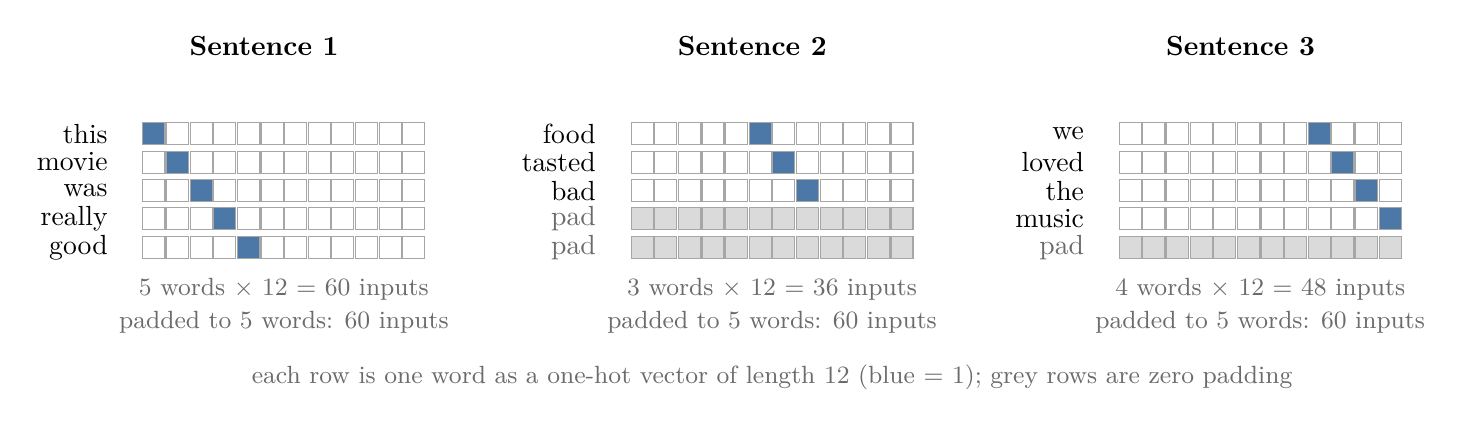
\begin{tikzpicture}[sq/.style={draw=cgrey!60, minimum size=0.28cm, inner sep=0pt, line width=0.4pt}]
  % vocabulary of 12 words, in this order
  % 1 this 2 movie 3 was 4 really 5 good 6 food 7 tasted 8 bad 9 we 10 loved 11 the 12 music
  % \sent{xshift}{title}{list of word:index}{number of words}{input size before padding}
  \newcommand{\sent}[5]{%
    \begin{scope}[xshift=#1cm]
      \node[font=\sffamily\bfseries] at (1.7, 0.75) {#2};
      \foreach \w/\k [count=\r] in {#3} {
        \node[anchor=east, font=\sffamily] at (-0.15, -0.36*\r) {\w};
        \foreach \c in {1,...,12} {
          \ifnum\c=\k \node[sq, fill=cblue] at (0.3*\c, -0.36*\r) {};
          \else \node[sq, fill=white] at (0.3*\c, -0.36*\r) {}; \fi }}
      \pgfmathtruncatemacro{\pad}{5-#4}
      \ifnum\pad>0
        \foreach \r in {1,...,\pad} {
          \pgfmathtruncatemacro{\rr}{#4+\r}
          \node[anchor=east, font=\sffamily, text=cgrey] at (-0.15, -0.36*\rr) {pad};
          \foreach \c in {1,...,12} \node[sq, fill=cgrey!25] at (0.3*\c, -0.36*\rr) {};}
      \fi
      \node[note, align=center] at (1.95, -2.55) {#4 words $\times$ 12 = #5 inputs\\[1pt] padded to 5 words: 60 inputs};
    \end{scope}}
  \sent{0}{Sentence 1}{this/1, movie/2, was/3, really/4, good/5}{5}{60}
  \sent{6.2}{Sentence 2}{food/6, tasted/7, bad/8}{3}{36}
  \sent{12.4}{Sentence 3}{we/9, loved/10, the/11, music/12}{4}{48}
  \node[note] at (8.15, -3.45) {each row is one word as a one-hot vector of length 12 (blue = 1); grey rows are zero padding};
\end{tikzpicture}
\end{document}
